\chapter{Conceitos Básicos}
\label{chapter:basicConcepts}



%----------NOTATION
\section{Algumas palavras sobre a notação}

Um dos príncipais objectivos neste texto é de reunir, corrigir, rever e homogenizar toda a informação existente relacionada com os mecanismos internos da cripto-moeda Monero. E ao mesmo tempo oferecer os detalhes suficientes, para apresentar a matéria de uma forma única e construtiva.

Entre outras importantes convenções, o seguinte foi usado :

\begin{itemize}
\item  letra minúscula para inteiros, representações de bits, strings e valores simples.
\item letra maiúscula para pontos em curvas elípticas e ou valores complexos.
\end{itemize}

Para itens com um significado especial, tentámos, o mais possível, usar sempre os mesmos símbolos. Por exemplo um gerador de curva e sempre denotado como \(G\), e a sua ordem é \(l\). Chaves privadas/públicas são denotadas usualmente por \(k/K\) respectivamente.
\\

Para além disso tentámos ser {\em conceptuais} na nossa presentação de algoritmos e esquemas. Um leitor com experiência em ciência da computação pode sentir que não foram esplicadas questões como a representação de bits de alguns itens, ou como executar certas operações. Para mais estudantes de matemática podem considerar que não foram dadas esplicações de algebra abstracta.   

%Beyond that, we have aimed at being {\em conceptual} in our presentation of algorithms and schemes. A reader with a computer science background may feel we have neglected questions like the bit representation of items, or, in some cases, how to carry out concrete operations. Moreover, students of mathematics may find we disregarded explanations of abstract algebra.

Contudo, isto não é visto como uma perda. Um simples objecto como um inteiro ou uma string (lista de characteres) pode sempre ser representado como uma lista de bits. A assim chamada `endianness' raramente é relevante, e é maioritariamente uma convenção nos nossos algoritmos. 
%However, we don’t see this as a loss. A simple object such as an integer or a string can always be represented by a bit string. So-called `endianness' is rarely relevant, and is mostly a matter of convention for our algorithms.
%\footnote{In computer memory, each byte is stored in its own address (an address is akin to a numbered slot, which a byte can be stored in). A given `word' or variable is referenced by the lowest address of its bytes. If variable $x$ has 4 bytes, stored in addresses 10-13, address 10 is used to find $x$. The way bytes of $x$ are organized in its set of addresses depends on {\em endianness}, although each individual byte is always and everywhere stored the same way within its address. Basically, which end of $x$ is stored in the reference address? It could be the {\em big end} or {\em little end}. Given $x = $ 0x12345678 (hexadecimal, 2 hexadecimal digits occupy 1 byte e.g. 8 binary digits a.k.a. bits), and an array of addresses \{10, 11, 12, 13\}, the big endian encoding of $x$ is \{12, 34, 56, 78\} and the little endian encoding is \{78, 56, 34, 12\}. \cite{endianness}}

Pontos de curva elíptica são normalmente denotados por pares \((x, y)\), e podem como tal ser representados por dois inteiros. Contudo, no mundo da criptografia é comum aplicar técnicas de compressão nos pontos. O que permite representar um ponto somente através de uma coordinada. Ao abordar estes conceitos tal informação torna-se secundária, neste case assume-se no entanto compressão de pontos de curva elíptica. 

As funções hash\marginnote{src/crypto/ {\tt keccak.c}} são aqui também referidas de forma livre e sem declarar algoritmos específicos. No caso de Monero trata-se de uma variante de \(\mathit{Keccak}\), mas como não é relevante para a teoria nao será explicitamente definido\footnote{\label{kekkak_note} O algoritmo da função hash Keccak é a base para o standard NIST {\em SHA-3} \cite{nist-sha3}.}.
%The Keccak hashing algorithm forms the basis for the NIST standard {\em SHA-3} \cite{nist-sha3}.}

Uma função de dispersão criptográfica ou função hash criptográfica, será daqui em diante simplesmente `função hash' ou também `hash'. Tais funções têm como entrada uma mensagem $\mathfrak{m}$ de comprimento variável, e devolvem como resultado uma hash $h$ de comprimento fixo. Para qualquer entrada, qualquer resultado é equiprovável. Funções hash são difíceis de inverter, possuem uma característica interessante conhecida como o {\em efeito avalanche} o que pode causar que duas entradas muito semelhantes produzam hashes muito diferentes e é também difícil encontrar duas mensagem de entrada que resultem na mesma hash. 

Funções hash irão ser aplicadas a inteiros, strings, pontos de curva ou combinações destes objectos. Estas occurências devem ser interpretadas como hashes de representações binárias, ou concatenações de tais representações. Dependendo do contexto, a hash resultante será numérica, uma sequência de bits, ou até um ponto de curva. Mais detalhes sobre o mesmo serão dados quando necessário.

%----------MODULAR ARITHMETIC
\section{Aritmética modular}
\label{sec:modular-arithmetic}

A maioria da criptografia moderna começa com aritmética modular, e assim com a operação de modulus (denotado por `mod'). Aqui só é de interesse o modulus positivo, que devolve sempre um inteiro positivo.

O modulus positivo é similar ao resto da divisão inteira.
Formalmente, o modulus positivo é definido como $c = a \pmod b$ tal que $a=bx+c$, em que $0\leq{c}<{b}$. Sendo $x$ um inteiro que é descartado.

Note-se que, se $a \leq n$, $-a \pmod n$ é o mesmo que $n - a$.


\subsection{adição e multiplicação modular}
\label{subsec:modular-addition-multiplication}

Na ciência da computação é importante evitar números enormes ao executar operações aritméticas. Por exemplo se temos $29+87 \pmod{99}$ e não são permitidas variáveis com mais de 3 ou 4 digitos (tal como $116 = 29+87$), então não podemos calcular $116 \pmod{99} = 17$ directamente.

Seja que $c = a+b \pmod n$, em que $a$ e $b$ são ambos menos do que o modulus $n$, podemos fazer o seguinte:
\begin{itemize}
	\item Calcule $x = n-a$. Se $x > b$ então $c = a+b$, se não $c = b - x$.
\end{itemize}

Podemos utilizar adição modular para executar multiplicação modular ($a*b \pmod n = c$) com um algoritmo chamado `double-and-add'. Eis um exemplo, queremos calcular $7*8 \pmod 9 = 2$. O que é o mesmo que :
\[7*8 = 8+8+8+8+8+8+8 \pmod 9\]

Isso é repartido em grupos de dois :
\[(8+8) + (8+8) + (8+8) + 8\]

Novamente, em grupos de dois : 
\[[(8+8) + (8+8)] + (8+8) + 8\]

O número total de operações $+$ decresce de 6 a 4 porque só temos de calcular $(8+8)$ uma vez.
\footnote{O efeito de duplica-e-adiciona torna-se aparente com números grandes. Por exemplo, com $2^{15} * 2^{30}$ adição normal iria requerer por volta de $2^{15}$ $+$ operações, enquanto que duplica-e-adiciona só requer 15!}\\ 
%The effect of double-and-add becomes apparent with large numbers. For example, with $2^{15} * 2^{30}$ straight addition would require about $2^{15}$ $+$ operations, while double-and-add only requires 15!}\\

Duplica-e-adiciona é implementado ao converter o primeiro número $a$ para binário, depois passando pelo vector binário, duplicando e adicionando.

%Double-and-add is implemented by converting the first number (the `multiplicand' $a$) to binary (in our example, 7 $\rightarrow$ [0111]), then going through the binary array and doubling and adding. 

Seja um vector $V = [0111]$ indexado com 3,2,1,0. 
%Let's make an array $A = [0111]$ and index it 3,2,1,0.
\footnote{Isto é conhecido como `LSB 0', do inglés :{\em least significant bit}, o bit menos significante que tem o index 0. No resto deste capítulo irá-se usar `LSB 0', como notação para esse bit. Trata-se aqui de clareza e não de convenções precisas.} 
%This is known as `LSB 0' numbering, since the least significant bit has index 0. We will use `LSB 0' for the rest of this chapter. The point here is clarity, not accurate conventions.} 
V[0] = 1 é o primeiro elemento de V e é o bit menos significante. A[0] = 1 é o primeiro elemento de A e é o bit menos significante. Existem mais duas variáveis, uma de resultado, que no início é : $r = 0$. E uma variável de soma, que no início é : $s = b$. Segue-se este algoritmo :   
%A[0] = 1 is the first element of A and is the least significant bit. We set a result variable to be initially $r = 0$, and set a sum variable to be initially $s = 8$ (more generally, we start with $s = b$). We follow this algorithm:
\begin{enumerate}
	\item Itera-se através de : $i = (0,...,A_{size} - 1)$
	\begin{enumerate}
		\item Se A[i] == 1, então $r = r + s \pmod n$.
		\item Calcula-se $s = s + s \pmod n$.
	\end{enumerate}
	\item Usa-se finalmente $r$: $c = r$.
\end{enumerate}

Por exemplo $7*8 \pmod 9$, esta sequência acontece :
\begin{enumerate}
	\item $i = 0$
	\begin{enumerate}
		\item A[0] = 1, então $r = 0 + 8 \pmod 9$ = 8
		\item $s = 8 + 8 \pmod 9$ = 7
	\end{enumerate}
	\item $i = 1$
	\begin{enumerate}
		\item A[1] = 1, então $r = 8 + 7 \pmod 9$ = 6
		\item $s = 7 + 7 \pmod 9$ = 5
	\end{enumerate}
	\item $i = 2$
	\begin{enumerate}
		\item A[2] = 1, então $r = 6 + 5 \pmod 9$ = 2
		\item $s = 5 + 5 \pmod 9$ = 1
	\end{enumerate}
	\item $i = 3$
	\begin{enumerate}
		\item A[3] = 0, então $r$ fica o mesmo
		\item $s = 1 + 1 \pmod 9$ = 2
	\end{enumerate}
	\item e o resultado é : $r = 2$
\end{enumerate}


\subsection{Exponenciação modular}

Claramente $8^7 \pmod 9 = 8*8*8*8*8*8*8 \pmod 9$. Da mesma forma que duplica-e-adiciona, pode-se também levar-ao-quadrado-e-multiplicar. Para $a^e \pmod{n}$ :
%Just like double-and-add, we can do square-and-multiply. For $a^e \pmod{n}$:
\begin{enumerate}
%	\item Define-se $e_{scalar} \rightarrow e_{binário}$; $A = [e_{binário}]$; $r = 1$; $m = a$
	\item Itera-se através de : $i = (0,...,A_{size} - 1)$
	\begin{enumerate}
		\item Se A[i] == 1, então $r = r * m \pmod n$.
		\item Calcula-se $m = m * m \pmod n$.
	\end{enumerate}
	\item Usa-se o $r$ final, como resultado.
\end{enumerate}


\subsection{Inversa multiplicativa modular}

As vezes precisa-se de $1/a \pmod n$, ou por outras palavras $a^{-1} \pmod n$. A inversa de algo vezes sí próprio é por definição 1 (identidade). Por exemplo : $0.25 = 1/4$, e depois $0.25*4 = 1$.  

%Sometimes we need $1/a \pmod n$, or in other words $a^{-1} \pmod n$. The inverse of something times itself is by definition one (identity). Imagine $0.25 = 1/4$, and then $0.25*4 = 1$.\\

Em aritmética modular, para $a$ e $n$ relativamente primos : 
\begin{align*} 
\\c = a^{-1} \pmod{n},
\\a c \equiv 1 \pmod{n},\ 0 \leq c < n. 
\end{align*}

%In modular arithmetic, for $c = a^{-1} \pmod{n}$, $a c \equiv 1 \pmod{n}$ for $0 \leq c < n$ and for $a$ and $n$ relatively prime.

\footnote{Na equação $a \equiv b \pmod{n}$, $a$ é {\em congruente} a $b \pmod{n}$, o que só significa \(a \pmod{n} = b \pmod{n}\).}
%In the equation $a \equiv b \pmod{n}$, $a$ is {\em congruent} to $b \pmod{n}$, which just means \(a \pmod{n} = b \pmod{n}\).} 
Relativamente primo significa que eles não partilham nenhum divisor comum excepto 1 (a fracção $a/n$ não pode ser reduzida ou simplificada).
%Relatively prime means they don't share any divisors except 1 (the fraction $a/n$ can't be reduced/simplified).

Podemos usar leva-ao-quadrado-e-multiplica para calcular a inversa multiplicativa quando $n$ é um número primo por causa do {\em pequeno teorema de Fermat} :
%We can use square-and-multiply to compute the modular multiplicative inverse when $n$ is a prime number because of {\em Fermat's little theorem}:
\footnote{\label{inverse_rule_note}A inversa multiplicativa modular tem uma regra que diz :
Se $a c \equiv b \pmod{n}$ com $a$ e $n$ relativamente primos, então a solução para esta congruência linear é dada por \(c = a^{-1} b \pmod{n}\).}\cite{wiki-modular-arithmetic}\\
Isto significa que se pode fazer :
$c = a^{-1} b \pmod n \rightarrow ca \equiv b \pmod n \rightarrow a \equiv c^{-1} b \pmod n$
\begin{align*} 
    a^{n-1} &\equiv 1 \pmod{n} \\
    a*a^{n-2} &\equiv 1 \pmod{n} \\
    c \equiv a^{n-2} &\equiv a^{-1} \pmod{n}
\end{align*}


\iffalse

The modular multiplicative inverse has a rule stating:\\
{\em If $a c \equiv b \pmod{n}$ with $a$ and $n$ relatively prime, the solution to this linear congruence is given by \(c = a^{-1} b \pmod{n}\).}\cite{wiki-modular-arithmetic}\\
It means we can do $c = a^{-1} b \pmod n \rightarrow ca \equiv b \pmod n \rightarrow a \equiv c^{-1} b \pmod n$.}\vspace{.175cm}
\begin{align*} 
    a^{n-1} &\equiv 1 \pmod{n} \\
    a*a^{n-2} &\equiv 1 \pmod{n} \\
    c \equiv a^{n-2} &\equiv a^{-1} \pmod{n}
\end{align*}

\fi

Mais geralmente (e mais rapidamente), o algoritmo extendido de euclides \cite{extended-euclidean}, também é capaz de encontrar inversas modulares.
%More generally (and more rapidly), the so-called `extended Euclidean algorithm' \cite{extended-euclidean} can also find modular inverses.


\subsection{Equações modulares}
\label{subsec:modular-equations}

Seja uma equação $c = 3*4*5 \pmod 9$. Dada uma operação binária $\circ$ (por exemplo, $\circ = *$) entre duas espressões $A$ e $B$:\vspace{.175cm} 
%Suppose we have an equation $c = 3*4*5 \pmod 9$. Computing this is straightforward. Given some operation $\circ$ (for example, $\circ = *$) between two expressions $A$ and $B$:\vspace{.175cm}
\[(A \circ B)\pmod{n} = {[A\pmod {n}] \circ [B\pmod{n}]}\pmod{n}\]

Neste exemplo, declara-se $A = 3*4$, $B = 5$, e $n = 9$:\vspace{.175cm}
\begin{align*}
(3*4 * 5) \pmod{9} &= {[3*4 \pmod {9}] * [5 \pmod{9}]} \pmod{9} \\
				   &= [3]*[5] \pmod 9 \\
				 c &= 6
\end{align*}

Agora pode-se também fazer subtração modular : \vspace{.175cm}
%Now we have a way to do modular subtraction.\vspace{.175cm}
\begin{align*}
A - B \pmod n &\rightarrow A + (-B) \pmod n \\
			  &\rightarrow {[A \pmod {n}] + [-B \pmod{n}]} \pmod{n}
\end{align*}\\

O mesmo princípio aplica-se a algo como $x = (a-b*c*d)^{-1} (e*f+g^{h}) \pmod n$.
%The same principle would apply to something like $x = (a-b*c*d)^{-1} (e*f+g^{h}) \pmod n$.
\iffalse
\footnote{The modulus of large numbers can exploit modular equations. It turns out $254 \pmod {13} \equiv 2*10*10 + 5*10 + 4 \equiv (((2)*10 + 5)*10 + 4) \pmod {13}$. An algorithm for $a \pmod n$ when $a > n$ is:
\begin{enumerate}
	\item Define $A \rightarrow [a_{decimal}]$; $r = 0$
	\item For $i = A_{size} - 1,...,0$
	\begin{enumerate}
		\item $r = (r*10 + A[i]) \pmod n$
	\end{enumerate}
	\item Use the final $r$ as result.
\end{enumerate}}
\fi


%----------ELLIPTIC CURVE CRYPTOGRAPHY
\section{Criptografia de curva elíptica}
\label{EllipticCurveCryptography}


\subsection{O que são curvas elípticas?}
\label{elliptic_curves_section}

Um\marginnote{{\tt fe}: field element} corpo finito \(\mathbb{F}_q\), no qual \(q\) é um número primo maior que 3, é o corpo formado pelo conjunto \(\{0, 1, 2, ..., q-1\}\). 
Adição e multiplicação \((+,  \cdot)\) e negação $(-)$ são calculados \( \pmod q\).
%Addition and multiplication \((+,  \cdot)\) and negation $(-)$ are calculated\( \pmod q\).

``Calculado\( \pmod q\)" significa que\( \pmod q\) é aplicado a qualquer instância de uma operação aritmética entre dois elementos pertencentes ao mesmo corpo, como também á sua negação. Por exemplo, dado um corpo finito \(\mathbb{F}_p\) com $p = 29$, $17+20=8$ porque $37 \pmod{29} = 8$. Como também, $-13 = -13 \pmod{29} = 16$.\\

Típicamente, uma curva elíptica com um dado par $(a,b)$ é definida como o conjunto de todos os pontos com coordinadas \((x, y)\) que satisfaçam a equação de {\em Weierstraß} \cite{Hankerson:2003:GEC:940321}:\footnote{\label{notation1}Notação: a frase $a \in \mathbb{F}$ significa que $a$ é um elemento no corpo finito $\mathbb{F}$.}\vspace{.175cm}
\[y^2 = x^3 + a x + b \quad \textrm{em que} \quad a, b, x, y \in \mathbb{F}_q\]

A cripto-moeda Monero utiliza uma curva especial pertencente a categoria de assim chamadas curvas {\em Twisted Edwards} \cite{Bernstein2008}, que são espressadas para um dado par $(a,d)$ :
%The cryptocurrency Monero uses a special curve belonging to the category of so-called {\em Twisted Edwards} curves \cite{Bernstein2008}, which are commonly expressed as (for a given $(a,d)$ pair):\vspace{.175cm}
\vspace{.175cm}
\[a x^2 + y^2 = 1 + d x^2 y^2 \quad \textrm{em que} \quad a, d, x, y \in \mathbb{F}_q \]

Iremos de seguida preferir esta forma de representação, a vantagem dada por esta forma é que certas primitivas criptográficas requerem assim menos operações aritméticas. O que resulta em algoritmos mais rápidos (veja-se Bernstein {\em et al.} em \cite{Bernstein2007} para mais detalhes).\\

Sejam \(P_1 = (x_1, y_1)\) e \(P_2 = (x_2, y_2)\) dois pontos pertencentes a uma curva elíptica {\em Twisted Edwards} (daqui em diante representado somente por uma CE). Definimos adição nos pontos $P_1 + P_2 = (x_1, y_1) + (x_2, y_2)$ como o ponto $P_3 = (x_3, y_3)$ tal que :\footnote{Típicamente, por razões de eficiência, pontos de curvas elípticas são convertidos em coordenadas projetivas\marginnote{src/crypto/ crypto\_ops\_ builder/ ref10Comm- entedComb- ined/\\ ge.h} antes de operações como a adição, de forma a evitar inversões dos pontos no dado corpo finito \cite{ecc-projective}}.
\vspace{.375cm}
\begin{align*}
x_3 & =  \frac{x_1 y_2 + y_1 x_ 2}{1 + d x_1 x_2 y_1 y_2}  \pmod{q} \\
\\
y_3 & =  \frac{y_1 y_2 - a x_1 x_2}{1 - d x_1 x_2 y_1 y_2} \pmod{q} 
\end{align*}
\\
Estas formulas para adição também se aplicam para duplicar um ponto, isto é, se \(P_1 = P_2\).\newline Para subtraír um ponto, inverte-se as suas coordinadas sobre o eixo y : $(x,y) \rightarrow (-x,y)$ \cite{Bernstein2008}, e depois aplica-se duplicar o ponto. Note-se que elementos negativos em $\mathbb{F}_q$, $-x$ são : $-x \pmod{q}$.
\\
Sempre que pontos de curva elíptica são adicionados, $P_3$ é um ponto que se mantêm na curva elíptica. Ou seja $x_3,y_3 \in \mathbb{F}_q$, e satisfazem a equação de CE. Daqui em diante diz-se que o ponto $x_3,y_3$ está em CE. Ou então, o Ponto $P$ em CE. 

%Whenever two curve points are added together $P_3$ is a point on the `original' elliptic curve, or in other words all $x_3,y_3 \in \mathbb{F}_q$ and satisfy the EC equation.
Um ponto $P$ em CE pode gerar um subgrupo de ordem (tamanho) $u$, ao multiplicar-se consigo próprio.\newline Por exemplo, um ponto $P$ pode formar um subgrupo de ordem 5 e conter os pontos $(0, P, 2P, 3P, 4P)$, cada um dos quais está em CE.  
%Each point $P$ in EC can generate a subgroup of order (size) $u$ out of some of the other points in EC using multiples of itself. For example, some point $P$’s subgroup might have order 5 and contain the points $(0, P, 2P, 3P, 4P)$, each of which is in EC. 

Neste caso em vez de $5P$, acontece o {\em ponto-no-infinito}, que é como se fosse a posição zero na curva elíptica.
%which is like the `zero’ position on an EC, and has coordinates $(0, 1)$.
%??? and has coordinates $(0, 1)$.
\footnote{Acontece que curvas elípticas tem uma estrutura de grupo {\em abeliana} para a operação de adição descrita aqui, desde que o ponto no infinito é o elemento de identidade. Uma definição concisa desta noção pode ser encontrada aqui : \url{https://brilliant.org/wiki/abelian-group/}.}
%It turns out elliptic curves have {\em abelian group} structure under the addition operation described, since their point-at-infinity's are identity elements. A concise definition of this notion can be found under \url{https://brilliant.org/wiki/abelian-group/}.}
Convenientemente, $5P + P = P$. Isto significa que o subgrupo é {\em cíclico}.
%!!! Não é bem, porque para um subgrupo ou grupo ser cíclico só pode ter um gerador ! 
%Conveniently, $5P + P = P$. This means the subgroup is {\em cyclic}.
%\footnote{\label{cyclical_note}Cyclic subgroup means, for $P$'s subgroup with order $u$, and with any integer $n$, $n P = [n \pmod{u}] P$. We can imagine ourselves standing on a point on a globe some distance from a `zero'th position, and each step we take moves us that distance. After a while, we will wind up back where we started, although it may take many revolutions before we land exactly on the original spot again. The number of steps it takes to land on the exact same spot is the `order' of the `stepping group', and all our footprints are unique points in that group. We recommend applying this concept to other ideas discussed here.}
\newline Todos os pontos $P$ em CE geram um subgrupo cíclico. Se $P$ gera um subgrupo cuja ordem é um número primo, então {\em todos os pontos} incluídos nesse subgrupo geram esse mesmo subgrupo (excepto claro o ponto no infinito).
No exemplo anterior tome-se múltiplos do ponto $2P$:\vspace{.175cm}  
\[2P, 4P, 6P, 8P, 10P \rightarrow 2P, 4P, 1P, 3P, 0\]

Outro exemplo: um subgrupo com ordem 6 $(0, P, 2P, 3P, 4P, 5P)$.\newline Tome-se múltiplos do ponto $2P$:\vspace{.175cm}
\[2P, 4P, 6P, 8P, 10P, 12P \rightarrow 2P, 4P, 0, 2P, 4P, 0\]
Aqui o subgrupo gerado pelo gerador $2P$ tem ordem 3. Desde que 6 não é primo, nem todos os membros do subgrupo, geram o próprio subgrupo.
%Here $2P$ has order 3. Since 6 is not prime, not all of its member points recreate the original subgroup.

Cada curva elíptica tem uma ordem $N$ igual ao número total de pontos que está em CE,
isto {\em incluí} o ponto no infinito, e a ordem de cada subgrupo que acontece, divide $N$  ({\em sem resto}). Isto é pelo theorema de Lagrange. Por outras palavras, imagine-se então um conjunto de todos os pontos em CE $\{0,P_1,...,P_{N-1}\}$. Se $N$ não é primo, então só existem subgrupos cuja ordem divide $N$.\newline Note-se no parágrafo anterior, que a ordem do subgrupo gerado por $2P$ tem ordem 3, e 3 divide 6.       

%Each EC has an order $N$ equal to the total number of points in the curve (including the point-at-infinity), and the orders of all subgroups generated by points are divisors of $N$ (by {\em Lagrange’s theorem}). We can imagine a set of all EC points $\{0,P_1,...,P_{N-1}\}$. If $N$ isn't prime, some points will make subgroups with orders equal to divisors of $N$.

Para encontrar a ordem, $u$, do subgrupo de qualquer ponto dado $P$ :
%To find the order, $u$, of any given point $P$'s subgroup:
\begin{enumerate}
    \item Encontra-se $N$ (e.g. usa-se o {\em algoritmo de Schoof}).
    \item Encontram-se todos os divisores de $N$.
    \item para cada divisor $n$ de $N$, calcula-se $n P$. 
    \item O menor $n$ tal que $n P = 0$ é a ordem $u$ do subgrupo. 
\end{enumerate} 

Curvas elípticas seleccionadas para criptografia tipicamente têm $N = hl$, em que $l$ é um número primo suficientemente grande (com 160 bits) e $h$ é o assim chamado {\em cofactor} que pode ser tão pequeno como 1 ou 2.
%ECs\marginnote{{\tt ge}: group element} selected for cryptography typically have $N = hl$, where $l$ is some sufficiently large (such as 160 bits) prime number and $h$ is the so-called {\em cofactor} which could be as small as 1 or 2.
\footnote{Curvas elípticas com cofactores pequenos permitem uma adição de ponto rápida etc . \cite{Bernstein2008}.}
%EC with small cofactors allow relatively faster point addition, etc. \cite{Bernstein2008}.} 
Um ponto no subgrupo de tamanho $l$ é usualmente seleccionado para ser o gerador $G$ como uma convenção. Para cada outro ponto $P$ nesse subgrupo existe um inteiro $0 < n \leq l$ que satisfaz $P = n G$. 

\iffalse
Seja que existe um ponto $P$ com ordem $N$, em que $N=h l$.\newline Qualquer outro ponto $P_i$, pode ser encontrado com um inteiro $n_i$ tal que :
\vspace{.375cm}
\begin{align*}
P_i=n_i P' .
\end{align*}
Desde que $N= h l$, existe só um subgrupo de tamanho $l$.
  
%Let's expand our understanding. Say there is a point $P'$ with order $N$, where $N=h l$. Any other point $P_i$ can be found with some integer $n_i$ such that $P_i=n_i P'$.

%If $P_1=n_1 P'$ has order $l$, any $P_2=n_2 P'$ with order $l$ must be in the same subgroup as $P_1$ because $l P_1=0 = l P_2$, and if $l(n_1 P') \equiv l(n_2 P') \equiv N P'=0$, then $n_1$ \& $n_2$ must both be multiples of $h$. 
%????
%Since $N= h l$, there are only $l$ multiples of $h$, implying only one subgroup of size $l$ is possible.

Put simply, the subgroup formed by multiples of $(h P')$ always contains $P_1$ and $P_2$. Furthermore, $h(n' P')=0$ when $n'$ is a multiple of $l$, and there are only $h$ such variations of $n' \pmod N$ (including the point at infinity for $n' = hl$) because when $n' = h l$ it cycles back to 0: $h l P' = 0$. So, there are only $h$ points $P$ in EC where $h P$ will equal 0.

A similar argument could be applied to any subgroup of size $u$. Any two points $P_1$ and $P_2$ with order $u$ are in the same subgroup, which is composed of multiples of $(N/u) P'$.
\\ \newline
With this new understanding it is clear we can use the following algorithm to find (non-point-at-infinity) points in the subgroup of order $l$:
\begin{enumerate}
    \item Find $N$ of the elliptic curve EC, choose subgroup order $l$, compute $h=N/l$.
    \item Choose a random point $P'$ in EC.
    \item Compute $P=h P'$.
    \item If $P=0$ return to step 2, else $P$ is in the subgroup of order $l$.
\end{enumerate}

\fi


Calcular o produto escalar entre qualquer inteiro $n$ e qualquer ponto $P$, $nP$, não é difícil.\newline Ao contrário de encontrar $n$ dados dois pontos $P_1$ e $P_2$ tal que : 
\vspace{.375cm}
\begin{align*}
P_1 = n P_2
\end{align*}
o que é consenso, de ser difícil, computacionalmente infazível.\newline É isto que se chama o {\em problema do logaritmo discreto} (PLD).\newline Multiplicação escalar pode como tal ser vista como uma função unidireccional. Isto permite o uso de curvas elípticas para o fim de criptografia. Não existe até á data, alguma equação, esquema ou algoritmo para resolver $n$ na equação $P_1 = n P_2$ . Ou seja mesmo com todos os computadores do mundo a tentarem resolver para $n$, só depois de milhões de anos é que uma solução seria encontrada. Existe um inteiro, $\gamma$ que é central em Monero, que ninguêm conhece e que está protegido pelo PLD (secção \ref{sec:pedersen_monero}).     
%---> chapter of pedersen commitments .
%\marginnote{{\tt sc}: scalar}  is thought to be computationally hard. By analogy to modular arithmetic, this is often called the {\em discrete logarithm problem} (DLP). Scalar multiplication can be seen as a {\em one-way function}, which paves the way for using elliptic curves for cryptography.
%\footnote{No known equation or algorithm can efficiently (based on available technology) solve for $n$ in $P_1 = n P_2$, meaning it would take many many years to unravel just one scalar product.}

O produto escalar $nP$ é equivalente a $(((P+P)+(P+P))+(P+P))…{n\ vezes})$. Apesar de não ser todas as vezes o mais efficiente, pode-se utilizar duplica-e-adiciona como na secção \ref{subsec:modular-addition-multiplication}, para obter a soma $R = n P$.  

% Though not always the most efficient approach, we can use double-and-add like in Section \ref{subsec:modular-addition-multiplication}. To get the sum $R = n P$, remember we use the $+$ point operation discussed in Section \ref{elliptic_curves_section}.

\begin{enumerate}
	\item Define-se $n_{scalar} \rightarrow n_{binary}$; $A = [n_{binary}]$; $R = 0$, 
o ponto no infinito; $S = P$
	\item Itera-se sobre: $i = (0,...,A_{size} - 1)$
	\begin{enumerate}
		\item Se A[i] == 1, então R += S.
		\item Computa-se S += S.
	\end{enumerate}
	\item Usa-se o R final como resultado.
\end{enumerate}



Note-se que escalares para pontos no subgrupo de tamanho $l$, são membros do corpo finito $\mathbb{F}_l$. Isto significa que a aritmética entre escalares é mod $l$.

%Note that EC scalars for points in the subgroup of size $l$ (which we will be using henceforth) are members of the finite field $\mathbb{F}_l$. This means arithmetic between scalars is mod $l$.


\subsection{Criptografia de chave pública com curvas elípticas}
\label{ec:keys}
%Algoritmos de criptografia de chave pública, são comparáveis a aritmética modular.   
%Public key cryptography algorithms can be devised in a way analogous to modular arithmetic.
%??? what

Seja \(k\) um número aleatório escolhido tal que \(0 < k < l\). Chama-se a este número uma {\em chave privada}. Também dito como uma chave secreta, abrevia-se então 
\(K\) = chave pública, \(k\) = chave secreta.      
%Let \(k\) be a randomly selected number satisfying \(0 < k < l\), and call it a {\em private key}.
%\footnote{The private key is sometimes known as a {\em secret key}. This lets us abbreviate: pk = public key, sk = secret key.} 
Calcula-se então a {\em chave pública} \(K\) com o produto escalar \(k G = K\).
Devido ao PLD não podemos facilmente deduzir \(k\) de \(K\) sabendo \(G\).
Isto permite o uso standard de algoritmos de criptografia de chave pública.

%Due to the {\em discrete logarithm problem} (DLP) we cannot easily deduce \(k\) from \(K\) alone. This property allows us to use the values \((k, K)\) in standard public key cryptography algorithms.


\subsection{A troca de chaves tipo Diffie-Hellman com curvas elípticas}
\label{DH_exchange_section}

A troca básica tipo {\em Diffie-Hellman} \cite{Diffie-Hellman} de um segredo partilhado entre a {\em alice} e o {\em bob} acontece da seguinte maneira :   

%A basic {\em Diffie-Hellman} \cite{Diffie-Hellman} exchange of a shared secret between {\em Alice} and {\em Bob} could take place in the following manner:

\begin{enumerate}

	\item A alice e o bob geram as suas próprias chaves \((k_A, K_A) \textrm{ and } (k_B, K_B)\). Ambos publicam ou trocam as suas chaves públicas, e mantêm as suas chaves privadas para sí próprios.
%Alice and Bob generate their own private/public keys \((k_A, K_A) \textrm{ and } (k_B, K_B)\). Both publish or exchange their public keys, and keep the private keys for themselves.
    \item Claramente é verdade que : 
\vspace{.375cm}
\begin{align*}
S = k_A K_B = k_A k_B G = k_B k_A G = k_B K_A = S
\end{align*}


    A alice pode calcular privadamente \(S = k_A K_B\),\newline e o bob pode calcular privadamente \(S = k_B K_A\),\newline ambos podem utilizar este valor \(S\) como um segredo partilhado. 

%Alice could privately calculate \(S = k_A K_B\), and Bob \(S = k_B K_A\), allowing them to use this single value as a shared secret.

Se a alice quer enviar uma mensagem $m$ ao bob,
\newline ela calcula a hash do segredo partilhado $h = \mathcal{H}(S)$,
\newline depois $x = m + h$, e envia $x$ ao bob .

O bob também calcula $h = \mathcal{H}(S)$,
\newline depois $m = x - h$, e como tal, o bob aprende $m$.    

%For example, if Alice has a message $m$ to send Bob, she could hash the shared secret \(h = \mathcal{H}(S)\), compute $x = m + h$, and send $x$ to Bob. Bob computes $h' = \mathcal{H}(S)$, calculates $m = x - h'$, and learns $m$.
%\end{enumerate}   

Um observador externo não seria capaz de facilmente calcular o segredo partilhado devido ao `Problema Diffie-Hellman' (PDH), que diz que encontrar $S$ de $K_A$ e $K_B$ é consenso, de ser difícil, computacionalmente infazível. Da mesma forma o DLP previne que se possa descobrir $k_A$ ou $k_B$ sabendo $K_A$ e $K_B$ \footnote{Diz que o PDH é pelo menos tão difícil como o DLP, mas isto ainda não foi provado. \cite{diffie-hellman-problem}}
.

%An external observer would not be able to easily calculate the shared secret due to the `Diffie-Hellman Problem' (DHP), which says finding $S$ from $K_A$ and $K_B$ is very difficult. Also, the DLP prevents them from finding $k_A$ or $k_B$.

%The DHP is thought to be of at least similar difficulty to the DLP, although it has not been proven. \cite{diffie-hellman-problem}}


\subsection{Assinaturas tipo Schnorr e a transformada Fiat-Shamir} 
\label{sec:schnorr-fiat-shamir}

Em 1989 Claus-Peter Schnorr, publicou um agora famoso protocolo de autenticação interactivo \cite{schnorr-signatures}. Este foi generalizado por Maurer em 2009 \cite{simple-zk-proof-maurer}. O protocolo permite ao signatário provar que dada uma chave pública $K$ tem conhecimento da chave privada $k$, sem revelar alguma informação sobre ela \cite{Signatures2015BorromeanRS}. 

%In 1989 Claus-Peter Schnorr published a now-famous interactive authentication protocol \cite{schnorr-signatures}, generalized by Maurer in 2009 \cite{simple-zk-proof-maurer}, that allowed someone to prove they know the private key $k$ of a given public key $K$ without revealing any information about it \cite{Signatures2015BorromeanRS}. It goes something like this:
Ambas as partes conhecem a chave pública K e o gerador G bem como o grupo pertencente.\newline Acontece da seguinte forma :
\iffalse
\begin{enumerate}
	\item o provador gera um número aleatório \(\alpha \in_R \mathbb{Z}_l\),
%The prover generates a random integer \(\alpha \in_R \mathbb{Z}_l\),
%\footnote{\label{notation3_note}Notation: The $R$ in \(\alpha \in_R \mathbb{Z}_l\) means $\alpha$ is randomly selected from \(\{1,2,3,...,l-1\}\).\marginnote{src/crypto/ crypto.cpp {\tt random32\_ unbiased()}} In other words, $\mathbb{Z}_l$ is all integers$\pmod l$. We exclude `$l$' since the point-at-infinity is not useful here.} 
	\item calcula $\alpha G$, e envia $\alpha G$ ao verificador.
	\item O verificador gera um {\em desafio} aleatório $c \in_R \mathbb{Z}_l$  
    \item e envia $c$ ao provador.
    \item O provador calcula a {\em resposta} $r = \alpha + c*k$
    \item e envia $r$ ao verificador.
	\item O verificador calcula $R = r G$ e $R' = \alpha G + c*K$, e verifica se :
$R \stackrel{?}{=} R'$. 
%The verifier computes $R = r G$ and $R' = \alpha G + c*K$, and checks $R \stackrel{?}{=} R'$.
\end{enumerate}
\fi

\tikzstyle{note} = [rectangle, rounded corners, minimum width=3cm, minimum height=1cm,text centered, draw=black, fill=green!30]
\tikzstyle{process} = [rectangle, minimum width=3cm, minimum height=1cm, text centered, draw=black, fill=orange!30]
\tikzstyle{arrow} = [thick,->,>=stealth]

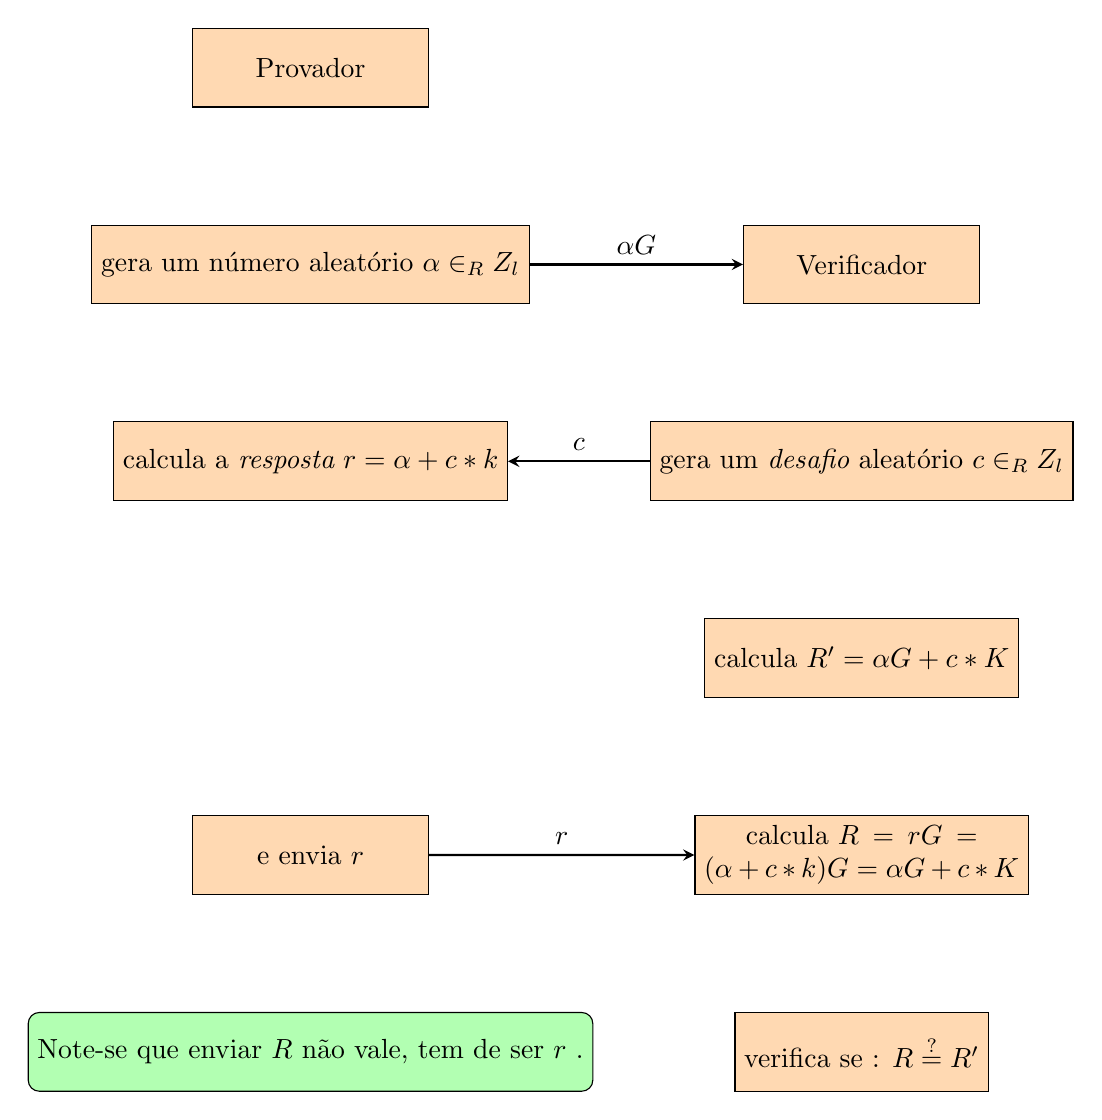
\begin{tikzpicture}[node distance=2cm]
\node (ver0) [process] {Provador};
\node (ver1) [process, below of=ver0, yshift=-0.5cm] {
gera um número aleatório 
\(\alpha \in_R \mathbb{Z}_l\)};
\node (ver2) [process, below of=ver1, yshift=-0.5cm] {calcula a {\em resposta} $r = \alpha + c*k$};
\node (ver3) [process, below of=ver2, yshift=-3.0cm] {e envia $r$};
\node (ver4) [note, below of=ver3, yshift=-0.5cm] {Note-se que enviar $R$ não vale, tem de ser $r$ .};
\node (pro0) [process, right of=ver1, xshift=5cm] { Verificador };
\node (pro1) [process, below of=pro0, yshift=-0.5cm] {gera um {\em desafio} aleatório $c \in_R \mathbb{Z}_l$};
\node (pro2) [process, below of=pro1, yshift=-0.5cm] {calcula $R' = \alpha G + c*K$};
\node (pro3) [process, below of=pro2, yshift=-0.5cm, text width=4cm] {calcula $R = r G = (\alpha + c*k)G = \alpha G + c*K$};
\node (pro4) [process, below of=pro3, yshift=-0.5cm] {verifica se : $R \stackrel{?}{=} R'$};
%\node (pro2c) [process, right of=pro2a, xshift=8cm] {Process 2b};
%\draw [arrow] (dec1) -- (pro2a);
\draw [arrow] (ver1) -- node[anchor=south] {$\alpha G$} (pro0);
\draw [arrow] (pro1) -- node[anchor=south] {$c$} (ver2);
\draw [arrow] (ver3) -- node[anchor=south] {$r$} (pro3);
%\draw [arrow] (pro2b) -- node[anchor=west] {$c$} (pro2c);
\end{tikzpicture}

Ou seja se $R = R'$, então o desafio foi {\em vencido} o que implica que o provador tinha de conhecer $k$ .\newline
O verificador pode calcular $R' = \alpha G + c*K$ antes do provador, assim oferecer $c$ é como dizer : "eu desafio-te a responderes com o logaritmo discreto de $R'$" .\newline Este desafio só pode ser vencido pelo provador que conhece $k$, que envia $r$, o que resolve a equação do lado do verificador (enp).        

%The verifier can compute $R' = \alpha G + c*K$ before the prover, so providing $c$ is like saying, ``I challenge you to respond with the discrete logarithm of $R'$." A challenge the prover can only overcome by knowing $k$ (except with negligible probability).
Se $\alpha$ foi escolhido de forma aleatória então $r$ está distribuído de forma aleatória \cite{SCOZZAFAVA1993313} e $k$ está seguro em termos da teoria da informação dentro de $r$ .\newline Segurança em termos da teoria da informação significa que mesmo um adversário com um poder de computação infinito não é capaz de a quebrar. 
%If $\alpha$ was chosen randomly by the prover then $r$ is randomly distributed \cite{SCOZZAFAVA1993313} and $k$ is information-theoretically secure within $r$ (it can still be found by solving the DLP for $K$ or $\alpha G$).
%???within $r$
%\footnote{\label{information_theoretic_note}A cryptosystem with information-theoretic security is one where even an adversary with infinite computing power could not break it, because they simply wouldn't have enough information.} 
Contudo, se um provador reutiliza $\alpha$ para provar o seu conhecimento de $k$...\newline Quem souber ambos os desafios em $r = \alpha + c*k$ and $r' = \alpha + c'*k$, pode calcular $k$ \footnote{Se o provador é um computador, o leitor pode imaginar que alguêm faz uma cópia do computador depois deste gerar $\alpha$, e depois apresentar cada cópia com um desafio diferente.} 
.  

%However, if the prover reuses $\alpha$ to prove his knowledge of $k$, anyone who knows both challenges in $r = \alpha + c*k$ and $r' = \alpha + c'*k$ can compute $k$ (two equations, two unknowns).
%If the prover is a computer, you could imagine someone `cloning'/copying the computer after it generates $\alpha$, then presenting each copy with a different challenge.}
\vspace{.175cm}%In security proofs, phrases like `forking lemma' and `rewind on success' are analagous to this cloning attack. See for example \cite{Liu2004}.
\[k = \frac{r-r'}{c-c'}\]

%Se o provador sabia $c$ do início  
%If the prover knew $c$ from the beginning (e.g. if the verifier secretly gave it to her), she could generate a random response $r$ and compute $\alpha G = r G - c K$. When she later sends $r$ to the verifier, she `proves' knowledge of $k$ without ever having to know it. Someone observing the transcript of events between prover and verifier would be none the wiser. The scheme is not {\em publicly verifiable}. \cite{Signatures2015BorromeanRS}\\
%??? why even mention this? Don't focus on how it does not work... but rather on how it does! 

No seu passo de desafio, o verificador oferece um número aleatório depois de receber $\alpha G$, o que o torna equivalente a uma {\em função aleatória}. Funções aleatórias, como funções de hash, são conhecidas como oráculos aleatórios. Em vez de ser o verificador a oferecer um desafio usa-se uma função hash.\newline Isto é conhecido como a {\em transformada de Fiat-Shamir} \cite{fiat-shamir-transform}, a prova torna-se não-interactiva e publicamente verificável \cite{Signatures2015BorromeanRS}. Da mesma forma como antes, o público conhece a chave pública K o gerador G e o grupo pertencente. A única diferença é que o desafio provêm de uma função hash conhecida também ao público.\newline Acontece da seguinte forma :
%In his role as challenger, the verifier spits out a random number after receiving $\alpha G$, making him equivalent to a {\em random function}. Random functions, such as hash functions, are known as random oracles because computing one is like requesting a random number from someone \cite{Signatures2015BorromeanRS}.
\footnote{Mais geralmente, ``[N]a criptografia... um oráculo é qualquer sistema que dá uma informação sobre um outro sistema, que de outra forma não estaria disponível."\cite{cryptographic-oracle}}
%More generally, ``[i]n cryptography... an oracle is any system which can give some extra information on a system, which otherwise would not be available."\cite{cryptographic-oracle}}
%Using a hash function, instead of the verifier, to generate challenges is known as a {\em Fiat-Shamir transform} \cite{fiat-shamir-transform}, because it makes an interactive proof non-interactive and publicly verifiable \cite{Signatures2015BorromeanRS}.
\footnote{O resultado de uma função hash criptográfica $\mathcal{H}$ está uniformemente distribuído entre o domínio de todos os resultados possíveis. Isto significa que, para um argumento $A$, $\mathcal{H}(A) \in^D_R \mathbb{S}_H$ em que $\mathbb{S}_H$ é o conjunto de resultados possíveis de $\mathcal{H}$. Usa-se $\in^D_R$ para indicar que a função é deterministicamente aleatória. $\mathcal{H}(A)$ produz sempre o mesmo resultado e esse resultado depende de um número aleatório.}
%The output of a cryptographic hash function $\mathcal{H}$ is uniformly distributed across the range of possible outputs. That is to say, for some input $A$, $\mathcal{H}(A) \in^D_R \mathbb{S}_H$ where $\mathbb{S}_H$ is the set of possible outputs from $\mathcal{H}$. We use $\in^D_R$ to indicate the function is deterministically random. $\mathcal{H}(A)$ produces the same thing every time, but its output is equivalent to a random number.}
\footnote{Note-se que provas não interactivas do tipo Schnorr (e as assinaturas) requerem o uso de um gerador fixo $G$, ou a inclusão desse gerador no desafio hash. Isto é conhecido como prefixo de chave e será apresentado mais tarde (secção  \ref{blsag_note} e \ref{sec:robust-key-aggregation}).} 
%Note that non-interactive Schnorr-like proofs (and signatures) require either use of a fixed generator $G$, or inclusion of the generator in the challenge hash. Including it that way is known as key prefixing, which we discuss a bit more later (Sections \ref{blsag_note} and \ref{sec:robust-key-aggregation}).}

\subsubsection*{Prova não interactiva}

\iffalse
\begin{enumerate}
	\item Gera-se um número aleatório $\alpha \in_R \mathbb{Z}_l$, e calcula-se $\alpha G$.  
	\item Calcula-se o desafio com uma função hash criptográficamente segura \(c = \mathcal{H}([\alpha G])\).
	\item Define-se a resposta $r = \alpha + c*k$.
	\item Publica-se o par de prova $(\alpha G, r)$.
\end{enumerate}

\subsubsection*{Verificação}

\begin{enumerate}
	\item Calcula-se o desafio: \(c' = \mathcal{H}([\alpha G])\).
	\item Calcula-se $R = r G$ e $R' = \alpha G + c'*K$.
	\item Se $R = R'$ então o provador tem de saber $k$ (enp).
\end{enumerate}
\fi

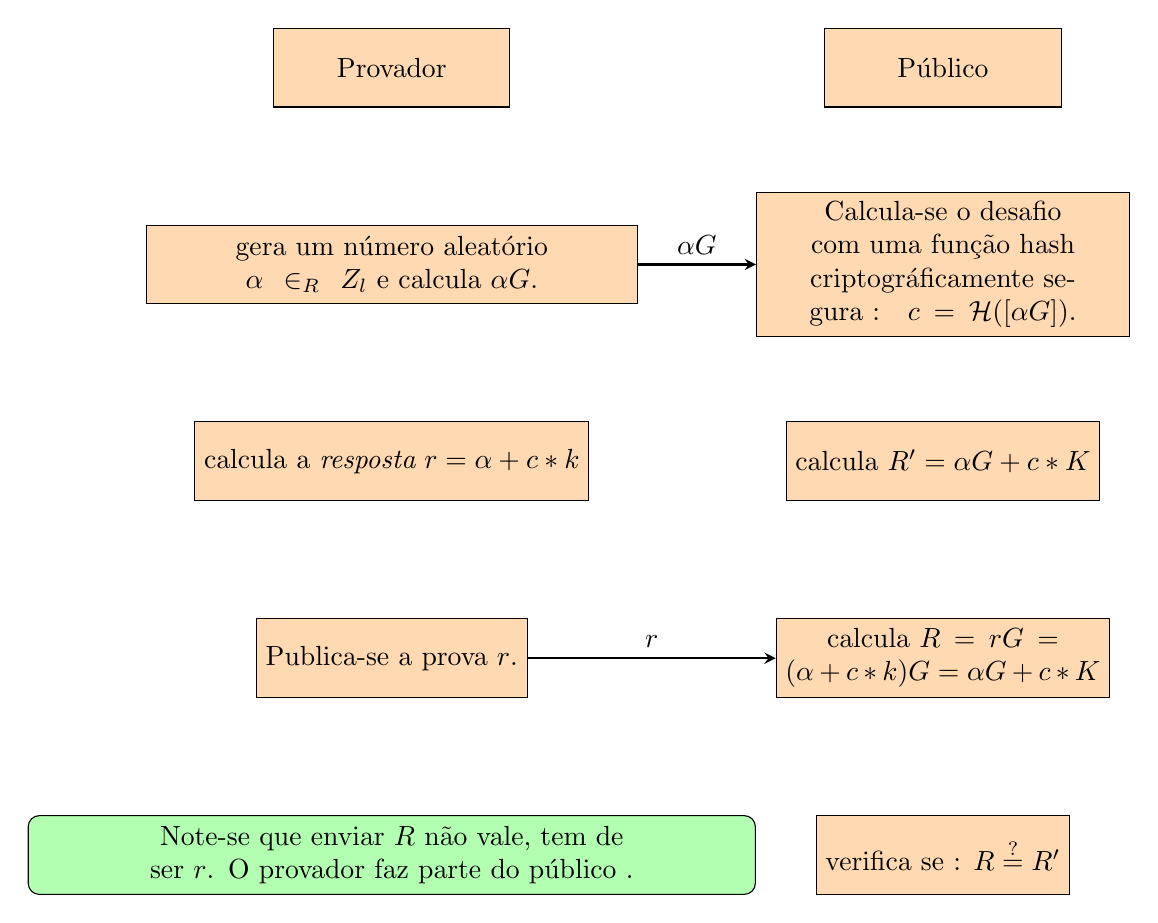
\begin{tikzpicture}[node distance=2cm]
\node (ver0_FS) [process] {Provador};
\node (ver1_FS) [process, below of=ver0_FS, yshift=-0.5cm, text width=6cm] {
gera um número aleatório 
\(\alpha \in_R \mathbb{Z}_l\) e calcula $\alpha G$.};
\node (ver2_FS) [process, below of=ver1_FS, yshift=-0.5cm] {calcula a {\em resposta} $r = \alpha + c*k$};
\node (ver3_FS) [process, below of=ver2_FS, yshift=-0.5cm] {Publica-se a prova $r$.};
\node (ver4_FS) [note, below of=ver3_FS, yshift=-0.5cm, text width=9cm] {Note-se que enviar $R$ não vale, tem de ser $r$. O provador faz parte do público .};
\node (pro0_FS) [process, right of=ver0_FS, xshift=5cm] { Público };
\node (pro1_FS) [process, right of=ver1_FS, xshift=5cm, text width=4.5cm] {Calcula-se o desafio com uma função hash criptográficamente segura :\quad \(c = \mathcal{H}([\alpha G])\).};
\node (pro2_FS) [process, below of=pro1_FS, yshift=-0.5cm] {calcula $R' = \alpha G + c*K$};
\node (pro3_FS) [process, right of=ver3_FS, xshift=5cm, text width=4cm] {calcula $R = r G = (\alpha + c*k)G = \alpha G + c*K$};
\node (pro4_FS) [process, below of=pro3_FS, yshift=-0.5cm] {verifica se : $R \stackrel{?}{=} R'$};
%\node (pro2c) [process, right of=pro2a, xshift=8cm] {Process 2b};
%\draw [arrow] (dec1) -- (pro2a);
\draw [arrow] (ver1_FS) -- node[anchor=south] {$\alpha G$} (pro1_FS);
%\draw [arrow] (pro1_FS) -- node[anchor=south] {$c$} (ver2_FS);
\draw [arrow] (ver3_FS) -- node[anchor=south] {$r$} (pro3_FS);
%\draw [arrow] (pro2b) -- node[anchor=west] {$c$} (pro2c);
\end{tikzpicture}

Ou seja se $R = R'$, então o desafio foi {\em vencido} o que implica que o provador tinha de conhecer $k$ . O provador faz parte do público, ou seja ele podia fazer este esquema sozinho. O que não faz muito sentido, provar a sí próprio que conhece $k$, é claro que o público não conhece $k$.

Parte importante de cada esquema de prova/assinatura são os requisitos computacionais para os verificar. Isto incluí o espaco para guardar as provas, e o tempo gasto para verificar. Neste esquema guarda-se um ponto de CE e um inteiro, mais a chave pública - outro ponto de CE. O tempo de verificação depende das operações de curva elíptica, desde que funções hash são rápidas de executar.   
\marginnote{src/ringct/ rctOps.cpp}


\subsection{Assinar mensagens}
\label{sec:signing-messages}

Típicamente, uma assinatura criptográfica é executada numa hash criptográfica de uma mensagem em vez de se assinar a própria mensagem. Isto facilita assinar mensagens de tamanho variável. Contudo aqui refere-se a mensagem com o seu símbolo $\mathfrak{m}$, de forma vaga, excepto quando definido se isso é o valor hash ou não.

%Typically, a cryptographic signature is performed on a cryptographic hash of a message rather than the message itself, which facilitates signing messages of varying size. However, in this report we will loosely use the term `message', and its symbol $\mathfrak{m}$, to refer to the message properly speaking and/or its hash value, unless specified.
Assinar mensagens faz parte da segurança na internet, o que deixa um recipiente de uma mensagem confiar que o seu conteúdo foi intendido pelo signatário. Um esquema comum de assinaturas é o de ECDSA. Veja-se \cite{ecdsa}, ANSI X9.62, e \cite{Hankerson:2003:GEC:940321}.  

%Signing messages is a staple of Internet security that lets a message's recipient be confident its content is as intended by the signer. One common signature scheme is called ECDSA. See \cite{ecdsa}, ANSI X9.62, and \cite{Hankerson:2003:GEC:940321}.

O esquema de assinaturas apresentado aqui é uma formulação alternativa da prova de Schnorr transformada. Pensar em assinaturas desta forma irá preparar-nos para explorar assinaturas em anel no próximo capítulo.   

%The signature scheme we present here is an alternative formulation of the transformed Schnorr proof from before. Thinking of signatures in this way prepares us for exploring ring signatures in the next chapter.

\iffalse

\subsubsection*{Assinatura}

Seja que a alice tem um par de chaves \((k_A, K_A)\). Para unequivocamente assinar uma mensagem arbitrária $\mathfrak{m}$, os seguintes passos são executados :

%Assume Alice has the private/public key pair \((k_A, K_A)\). To unequivocally sign an arbitrary message $\mathfrak{m}$, she could execute the following steps:

\begin{enumerate}
	\item Generate random number $\alpha \in_R \mathbb{Z}_l$, and compute $\alpha G$.
	\item Calculate the challenge using a cryptographically secure hash function, \(c = \mathcal{H}(\mathfrak{m},[\alpha G])\).
	\item Define the response $r$ such that $\alpha = r + c*k_A$. In other words, $r = \alpha - c*k_A$.
	\item Publish the signature $(c, r)$.
\end{enumerate}

\subsubsection*{Verificação}

Qualquer entidade terceira que saiba os parametros de CE, a assinatura $(c, r)$ e o methodo de assinatura, a mensagem $\mathfrak{m}$, a função hash e $K_A$ pode verificar a assinatura :

%Any third party who knows the EC domain parameters (specifying which elliptic curve was used), the signature $(c, r)$ and the signing method, $\mathfrak{m}$ and the hash function, and $K_A$ can verify the signature:

\begin{enumerate}
	\item Calcula-se o desafio: \(c' = \mathcal{H}(\mathfrak{m},[r G + c*K_A])\).
	\item Se $c = c'$ então a assinatura é válida.
\end{enumerate}

\fi


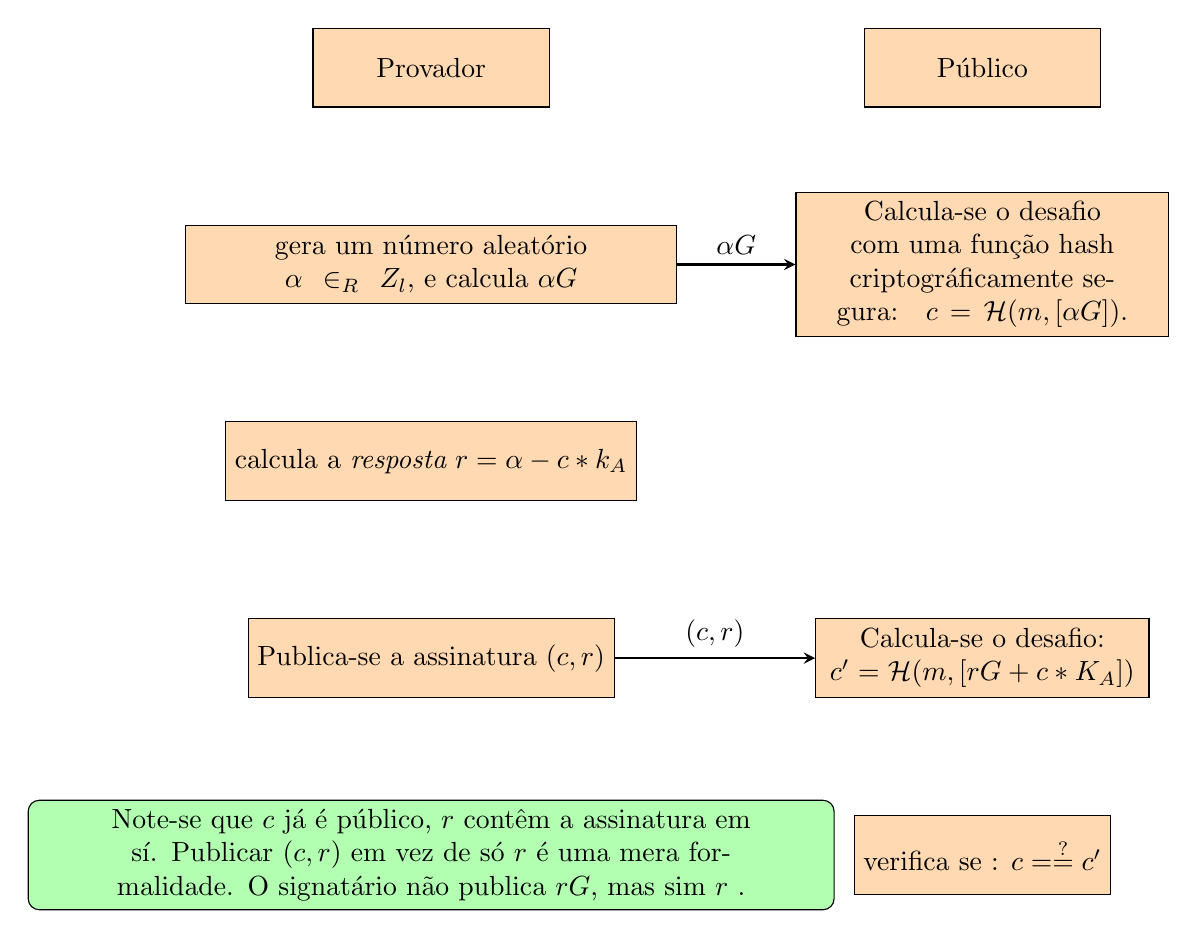
\begin{tikzpicture}[node distance=2cm]
\node (ver0_SM) [process] {Provador};
\node (ver1_SM) [process, below of=ver0_SM, yshift=-0.5cm, text width=6cm] {gera um número aleatório $\alpha \in_R \mathbb{Z}_l$, e calcula $\alpha G$};
\node (ver2_SM) [process, below of=ver1_SM, yshift=-0.5cm] {calcula a {\em resposta} $r = \alpha - c*k_A$};
\node (ver3_SM) [process, below of=ver2_SM, yshift=-0.5cm] {Publica-se a assinatura $(c, r)$};
\node (ver4_SM) [note, below of=ver3_SM, yshift=-0.5cm, text width=10cm] {Note-se que $c$ já é público, $r$ contêm a assinatura em sí. Publicar $(c, r)$ em vez de só $r$ é uma mera formalidade. O signatário não publica $rG$, mas sim $r$ .};
\node (pro0_SM) [process, right of=ver0_SM, xshift=5cm] { Público };
\node (pro1_SM) [process, right of=ver1_SM, xshift=5cm, text width=4.5cm] {Calcula-se o desafio com uma função hash criptográficamente segura:\quad \(c = \mathcal{H}(\mathfrak{m}, [\alpha G])\).};
%\node (pro2_SM) [process, below of=pro1_SM, yshift=-0.5cm, text width=4.5cm] {
%\(     r G &= (\alpha - c*k_A) G \\
%  	  	 &= \alpha G - c*K_A, então :    
%     \alpha G &= r G + c*K_A    \)
%};
\node (pro3_SM) [process, right of=ver3_SM, xshift=5cm, text width=4cm] {Calcula-se o desafio: \(c' = \mathcal{H}(\mathfrak{m},[r G + c*K_A])\)};
\node (pro4_SM) [process, below of=pro3_SM, yshift=-0.5cm] {verifica se : $c =  \stackrel{?}{=} c'$};
%\node (pro2c) [process, right of=pro2a, xshift=8cm] {Process 2b};
%\draw [arrow] (dec1) -- (pro2a);
\draw [arrow] (ver1_SM) -- node[anchor=south] {$\alpha G$} (pro1_SM);
%\draw [arrow] (pro1_FS) -- node[anchor=south] {$c$} (ver2_FS);
\draw [arrow] (ver3_SM) -- node[anchor=south] {$(c, r)$} (pro3_SM);
%\draw [arrow] (pro2b) -- node[anchor=west] {$c$} (pro2c);
\end{tikzpicture}

Se $c = c'$ então a assinatura é válida.
  
%In this signature scheme we store two scalars, and need one public EC key.

\subsubsection*{Funciona porque}

Isto provém do facto que 
%This stems from the fact that
\begin{align*}
       r &= \alpha - c*k_A \\
  	 r G &= (\alpha - c*k_A) G \\
  	 r G &= \alpha G - c*K_A \\
\alpha G &= r G + c*K_A \\
\mathcal{H}_n(\mathfrak{m},[\alpha G]) &= \mathcal{H}_n(\mathfrak{m},[r G + c*K_A]) \\
       c &= c' \\
\alpha G &= (\alpha - c*k_A) G + c*K_A\\
\marginnote{"dabra pokus!"}
\alpha G &= \alpha G - c*K_A + c*K_A\\
\alpha G &= \alpha G
\end{align*}

Portanto a alice criou $(c,r)$ em dependência de $\mathfrak{m}$ com posse de $k_A$ : 
\newline ela assinou a mensagem.\newline A probabilidade que outra pessoa sem posse de $k_A$, podia ter produzido $r$ é negligível, portanto um verificador confia que a mensagem não foi falsificada. 


Requisitos :

Neste esquema de assinatura guardam-se dois escalares, e uma chave pública de CE.

%Therefore the owner of $k_A$ (Alice) created $(c,r)$ for $\mathfrak{m}$: she signed the message. The probability someone else, a forger without $k_A$, could have made $(c,r)$ is negligible, so a verifier can be confident the message was not tampered with.



%----------CURVE ED25519
\section{Curva Ed25519}
\label{Ed25519_section}

Monero utiliza uma curva elíptica particular tipo {\em Twisted Edwards} para operações criptográficas, {\em Ed25519 }\ o \ {\em equivalente birational} \ da curva de\ {\em Montgomery} : {\em Curve25519}.  
%Monero uses a particular Twisted Edwards elliptic curve for cryptographic operations, {\em Ed25519}, the {\em birational equivalent}
\footnote{\label{birational_note}Sem dar mais detalhes, equivalência birational pode ser vista como um isomorfismo que usa termos rationais.} 
%Without giving further details, birational equivalence can be thought of as an isomorphism expressible using rational terms.} 
%of the Montgomery curve {\em Curve25519}.
Ambas as curvas {\em Curve25519} e {\em Ed25519} foram públicadas por Bernstein {\em et al.} \cite{Bernstein2008, Bernstein2012, Bernstein2007}.
%Both Curve25519 and Ed25519 were released by Bernstein {\em et al.} \cite{Bernstein2008, Bernstein2012, Bernstein2007}.
\footnote{Dr. Bernstein também desenvolveu um esquema de encriptação conhecido como ChaCha \cite{Bernstein_chacha,chacha-irtf}, que a implementação primária de Monero utiliza para encriptar \marginnote{src/wallet/ ringdb.cpp} certas informações sensitivas relacionadas com a carteira.}  

%also developed an encryption scheme known as ChaCha \cite{Bernstein_chacha,chacha-irtf}, which the primary Monero implementation uses to encrypt\marginnote{src/wallet/ ringdb.cpp} certain sensitive information related to users' wallets.}

A curva é definida sobre o corpo finito primo : 
\vspace{.175cm}
\begin{align*}
\mathbb{F}_{2^{255} - 19}
\end{align*}
através da seguinte equação : 
%The
\marginnote{src/crypto/ crypto\_ops\_ builder/ ref10Comm- entedComb- ined/\\ ge.h} %curve is defined over the prime field \(\mathbb{F}_{2^{255} - 19}\) (i.e. $q = 2^{255}-19$) by means of the following equation:
\vspace{.175cm}
\begin{align*}
-x^2 + y^2 = 1 - \frac{121665}{121666} x^2 y^2
\end{align*}

Esta curva faz juz a algumas preocupações da comunidade de criptografia.
%This curve addresses many concerns raised by the cryptography community.
\footnote{Mesmo se uma curva aparentemente não tem nenhums problemas de segurança criptográfica, é possível que a pessoa ou organização que criou essa curva conheça um aspecto ou característica que só acontece em curvas raras... Esta pessoa pode gerar imensas curvas diferentes que não têm nenhums erros conhecidos, mas que tem um erro escondido a terceiros. Se adicionalmente são necessárias explicações para cada parametro de curva, para que esta curva seja aceite na comunidade criptográfica, então torna-se ainda mais difícil encontrar curvas com tais fraquezas. A curva Ed25519 é conhecida como uma curva `fully rigid', o que significa que o processo de geração desta curva está completamente descrito. \cite{elliptic-curve-rigidity} }  

%Even if a curve appears to have no cryptographic security problems, it's possible the person/organization that created it knows a secret issue that only crops up in very rare curves. Such a person may have to randomly generate many curves in order to find one with a hidden weakness and no known weaknesses. If reasonable explanations are required for curve parameters, then it becomes even more difficult to find weak curves that will be accepted by the cryptographic community. Curve Ed25519 is known as a `fully rigid' curve, which means its generation process was fully explained. \cite{elliptic-curve-rigidity}} 
É bem sabido que algoritmos standard do NIST têm problemas\footnote{\label{NIST_note}National Institute of Standards and Technology, \url{https://www.nist.gov/}} 
.\newline Por exemplo, tornou-se recentemente claro que o algoritmo standard para gerar números aleatórios, a versão baseada em curvas elípticas, contêm uma potential porta de trás \cite{hales2014nsa}. Visto de uma perspectiva mais ampla, autoridades que emitem standards como o NIST levam a uma monocultura na criptografia, introdizindo um ponto de centralização. Um grande exemplo disto foi quando a NSA utilizou a sua influência sobre o NIST para enfraquecer um standard international de criptografia \cite{NSA-NIST}.   
%It is well known that NIST
%\footnote{\label{NIST_note}National Institute of Standards and Technology, \url{https://www.nist.gov/}} 
%standard algorithms have issues. For example, it has recently become clear the NIST standard random number generation algorithm PNRG (the version based on elliptic curves) is flawed and contains a potential backdoor \cite{hales2014nsa}. Seen from a broader perspective, standardization authorities like NIST lead to a cryptographic monoculture, introducing a point of centralization. A great example of this was illustrated when the NSA used its influence over NIST to weaken an international cryptographic standard \cite{NSA-NIST}.
A curva {\em Ed25519} não está sujeita a nenhums patentes (veja-se \cite{ECC-patents}), e a sua equipa desenvolveu \marginnote{src/crypto/ crypto\_ops\_ builder/} e adaptou algoritmos criptográficos com foco na eficiência\cite{Bernstein2007}.
%Curve Ed25519 is not subject to any patents (see \cite{ECC-patents} for a discussion on this subject), and the team behind it has
%developed\marginnote{src/crypto/ crypto\_ops\_ builder/} and adapted basic cryptographic algorithms with efficiency in mind \cite{Bernstein2007}.
Curvas do tipo {\em Twisted Edwards} têm uma ordem que se expressa como :
\vspace{.175cm}
\begin{align*}
N=2^c l ,
\end{align*}
em que $l$ é um número primo e $c$ é um inteiro positivo. No caso de Monero, a ordem é um número com 76 digitos, $l$ tem 253 bits \footnote{Isto significa que as chaves privadas em Ed25519 têm 253 bits.}: 
%Twisted Edwards curves have order expressible as \(N=2^c l\), where \(l\) is a prime number and \(c\) a positive integer. In the case of curve Ed25519, its order is a 76 digit number ($l$ is 253 bits):
%\footnote{This means private EC keys in Ed25519 are 253 bits.}
\vspace{.175cm}
\begin{align*}
2^3 \cdot 72370055773322622139731865630429942408\\57116359379907606001950938285454250989
\end{align*}
\marginnote{src/ringct/ rctOps.h {\tt curve- Order()}}


\subsection{Representação binária}
\label{binary_note}
Elementos de \(\mathbb{F}_{2^{255} - 19} \) estão codificados como inteiros de 256-bits, portanto podem ser representados com 32 bytes. Desde que cada elemento só requer 255 bits, o bit mais significante é sempre zero. 
%Elements of \(\mathbb{F}_{2^{255} - 19} \) are encoded as 256-bit integers, so they can be represented using 32 bytes. Since each element only requires 255 bits, the most significant bit is always zero.

%Consequently, any point in Ed25519 could be expressed using 64 bytes. By applying {\em point compression} techniques, described here below, however, it is possible to reduce this amount by half, to 32 bytes.
%??? expressed using 64 bytes ? or 32 ?

\subsection{Compressão de ponto elíptico}
\label{point_compression_section}

A curva Ed25519 tem a propriedade que os seus pontos podem ser facilmente comprimidos, portanto representar um ponto é possível com o espaço de só uma coordinada. Não iremos detalhar a matemática necessária para justificar isto, mas podemos dar uma breve esplicação de como isto funciona \cite{eddsa-ed25519-irtf}. A compressão de ponto foi primeiro descrito em \cite{Bernstein2012}, enquanto que o conceito foi primeiro introduzido em \cite{Miller:point-compression-origin}.

%The Ed25519 curve has the property that its points can be easily compressed, so that representing a point will consume only the space of one coordinate. We will not delve into the mathematics necessary to justify this, but we can give a brief insight into how it works \cite{eddsa-ed25519-irtf}. Point compression for the Ed25519 curve was first described in \cite{Bernstein2012}, while the concept was first introduced in \cite{Miller:point-compression-origin}.

Este esquema de compressão de ponto segue-se de uma transformação da equação de curva {\em Twisted Edwards}, (assumindo $a = -1$, o que é verdade para Monero) :
\begin{align*}
\\
x^2 = \frac{y^2-1}{d y^2+1} ,
\\
\end{align*}
em que $d = - \frac{121665}{121666}$ . Como tal existem dois valores possíveis para $x$ para cada $y$. Os elementos do corpo finito $x$ e $y$ são calculados $\pmod{q}$, por isso não existem valores negativos. No entanto, $\pmod{q}$ de $–x$ muda o valor entre par e impar desde que $q$ é impar. Por exemplo : $3 \pmod{5} = 3$, $-3 \pmod{5} = 2$. Por outras palavras, os elementos do corpo finito $x$ e $–x$ têm valores pares e impares diferentes.    
%This point compression scheme follows from a transformation of the Twisted Edwards curve equation (assuming $a = -1$, which is true for Monero): $x^2 = (y^2-1)/(d y^2+1)$,
%\footnote{Here $d = - \frac{121665}{121666}$.} 
%which indicates there are two possible $x$ values ($+$ or $-$) for each $y$. Field elements $x$ and $y$ are calculated$\pmod{q}$, so there are no actual negative values. However, taking$\pmod{q}$ of $–x$ will change the value between odd and even since $q$ is odd. For example: $3 \pmod{5} = 3$, $-3 \pmod{5} = 2$. In other words, the field elements $x$ and $–x$ have different odd/even assignments.
Seja um ponto de CE em que o seu $x$ é par, mas dado o seu valor $y$, a transformada da equação de curva resulta num número impar, então sabe-se que negar esse número irá dar-nos o $x$ correcto. Um bit consegue conter esta informação, e convenientemente a coordinada de $y$ tem um bit extra.

%???

%If we have a curve point and know its $x$ is even, but given its $y$ value the transformed curve equation outputs an odd number, then we know negating that number will give us the right $x$. One bit can convey this information, and conveniently the $y$ coordinate has an extra bit.

Seja que se quer comprimir um ponto \((x, y)\).
%Assume we want to compress a point \((x, y)\).

\begin{description}
	\item[Codificar] O bit mais significante de $y$ é posto a zero se $x$ é par, se não é posto a 1. O valor resultante $y’$ representa o ponto de curva CE.
%We\marginnote{src/crypto/ crypto\_ops\_ builder/ ref10Comm- entedComb- ined/\\ ge\_to- bytes.c} set the most significant bit of $y$ to 0 if $x$ is even, and 1 if it is odd. The resulting value $y’$ will represent the curve point.
	
	\item[Descodificar] \hfill
	    \begin{enumerate}
    	    \item Do ponto comprimido $y’$ copia-se o bit mais significante para uma variável $b$, Agora põe-se o bit mais significante de $y’$ de volta a zero, e obtêm-se outra vez o valor $y$ original.\marginnote{ge\_from- bytes.c}[2.05cm]    
%Retrieve\marginnote{ge\_from- bytes.c}[2.05cm] the compressed point $y’$, then copy its most significant bit to the parity bit $b$ before setting it to 0. Now it is the original $y$ again.
    	    \item Seja \(u = y^2-1 \pmod q\) e \(v = d y^2  + 1 \pmod q\). Isto significa $x^2 = u/v \pmod q$.
    	    \item Calcule\footnote{Desde que $q = 2^{255}-19 \equiv 5 \pmod{8}$, $(q-5)/8$ e $(q-1)/4$ são inteiros.} \(z = u v^3 (u v^7)^{(q-5)/8} \pmod q\).
            \begin{enumerate}
                \item Se \(v z^2 = u \pmod q\) então \(x' = z\).
                \item Se \(v z^2 = -u \pmod q\) então calcula-se \(x' = z*2^{(q-1)/4} \pmod q\).
            \end{enumerate}
            \item Usa-se o bit de paridade, se $b \ne$ do bit menos significante de $x'$ então \(x = -x' \pmod q\), se não \(x = x'\).
%Using the parity bit \(b\) from the first step, if $b \ne$ the least significant bit of $x'$ then  \(x = -x' \pmod q\), otherwise \(x = x'\).
            \item Resulta então o ponto descomprimido $(x,y)$.
%Return the decompressed point $(x,y)$.
	    \end{enumerate}
\end{description}

Implementações de Ed25519 (como em Monero) típicamente usam o gerador $G = (x,4/5)$ \cite{Bernstein2012}, em que x é par.

%Implementations of Ed25519 (such as Monero) typically use the generator $G = (x,4/5)$ \cite{Bernstein2012}, where x is the `even', or $b = 0$, variant based on point decompression of \(y = 4/5 \pmod q\).
%??? or $b = 0$, variant ?

\subsection{Algoritmo de assinatura EdDSA}
\label{EdDSA_section}

%Bernstein and his team have developed a number of basic algorithms based on curve Ed25519.\footnote{\label{group_ops_twisted_edwards_note}See\marginnote{src/crypto/ crypto\_ops\_ builder/ ref10Comm- entedComb- ined/} \cite{Bernstein2007} for efficient group operations in Twisted Edwards EC (i.e. point addition, doubling, mixed addition, etc). See \cite{curve25519} for efficient modular arithmetic.}
%!!!2
Com a intenção de ilustrar descreve-se uma alternativa optimizada e segura do esquema de ECDSA, que segundo os autores, permite produzir mais de 100 000 assinaturas por segundo com um processador Intel Xeon \cite{Bernstein2012}. O algoritmo também pode ser lido em {\em RFC8032} \cite{rfc8032}. Note-se que este esquema de assinaturas é do estilo Schnorr.  
%For illustration purposes we will describe a highly optimized and secure alternative to the ECDSA signature scheme which, according to the authors, allows producing over 100 000 signatures per second using a commodity Intel Xeon processor \cite{Bernstein2012}. The algorithm can also be found described in Internet RFC8032 \cite{rfc8032}. Note this is a very Schnorr-like signature scheme.
Entre outras coisas, em vez de gerar inteiros aleatórios cada vez, é usado um valor hash derivado da chave privada do signatário e da própria mensagem. Isto evita problemas de segurança relacionados com a implementação de geradores de números aleatórios. Outro objectivo deste algoritmo é de evitar o acesso a espaços secretos ou imprevisíveis em memória ram, o que previne assim chamados {\em ataques de cache temporais} \cite{Bernstein2012}. Aqui são esplicados por alto os passos executados pelo algoritmo. Uma descrição completa e uma implementação exemplo em Python pode ser encontrada em \cite{rfc8032}.

%Among other things, instead of generating random integers every time, it uses a hash value derived from the private key of the signer and the message itself. This circumvents security flaws related to the implementation of random number generators. Also, another goal of the algorithm is to avoid accessing secret or unpredictable memory locations to prevent so-called {\em cache timing attacks} \cite{Bernstein2012}.
%We provide here an outline of the steps performed by the algorithm. A complete description and sample implementation in the Python language can be found in \cite{rfc8032}. 

\subsubsection*{Assinatura}

\begin{enumerate}
	\item Seja \(h_k\) uma hash \(\mathcal{H}(k)\) da chave privada do signatário \(k\). Calcula-se \(\alpha\) como uma hash \(\alpha = \mathcal{H}(h_k, \mathfrak{m})\) da chave privada e da mensagem. Dependendo da implementação, $\mathfrak{m}$ pode ser a mensagem ou a sua hash \cite{rfc8032}.  

%Let \(h_k\) be a hash \(\mathcal{H}(k)\) of the signer's private key \(k\). Compute \(\alpha\) as a hash \(\alpha = \mathcal{H}(h_k, \mathfrak{m})\) of the hashed private key and message. Depending on implementation, $\mathfrak{m}$ could be the actual message or its hash \cite{rfc8032}.
	
	\item Calcula-se \(\alpha G\) e o desafio $ch = \mathcal{H}([\alpha G], K,  \mathfrak{m})$.

	\item Calcula-se a resposta \(r = \alpha + ch \cdot k \).
	
	\item A assinatura é o par \((\alpha G, r)\).
\end{enumerate}

\subsubsection*{Verificação}
A verificação procede da seguinte forma :

\begin{enumerate}
	\item Calcula-se \(ch' = \mathcal{H}([\alpha G], K,  \mathfrak{m})\).
	
	\item Se a seguinte equação é verdade :
\begin{align*}
2^c r G \stackrel{?}{=} 2^c \alpha G + 2^c ch'*K ,
\end{align*}
então a assinatura é válida.
\end{enumerate}

O termo $2^c$ vem da forma geral do algoritmo EdDSA (Bernstein {\em et al.}\cite{Bernstein2012}).  
%The $2^c$ term comes from Bernstein {\em et al.}’s general form of the EdDSA algorithm \cite{Bernstein2012}. According to that paper, though it isn’t required for adequate verification, removing $2^c$ provides stronger equations.
%???stronger ? 
A chave pública $K$ pode ser qualquer ponto de CE, mas só se quer usar os pontos no subgrupo do gerador $G$. Multiplicar pelo cofactor $2^c$ garante que todos os pontos estão nesse subgrupo. Alternativamente, pode-se verificar se $l K \stackrel{?}{=} 0$ o que só funciona se $K$ está dentro do subgrupo. Não se sabe de alguma fraqueza causada por estas precauções, e como iremos ver mais tarde, isto é um méthodo importante em Monero (secção \ref{blsag_note}).       

%The public key $K$ can be any EC point, but we only want to use points in the generator $G$'s subgroup. Multiplying by the cofactor $2^c$ ensures all points are in that subgroup. Alternatively, verifiers could check $l K \stackrel{?}{=} 0$, which only works if $K$ is in the subgroup. We do not know of any weaknesses caught by these precautions, though as we will see the latter method is important in Monero (Section \ref{blsag_note}).


\subsubsection*{Funciona porque}


\begin{align*}
2^c r G &= 2^c (\alpha + \mathcal{H}([\alpha G], K,  \mathfrak{m}) \cdot k) \cdot G\\
		&= 2^c \alpha G + 2^c \mathcal{H}([\alpha G], K,  \mathfrak{m}) \cdot K\\ 
2^c (\alpha + ch \cdot k) \cdot G &= 2^c \alpha G + 2^c \mathcal{H}([\alpha G], K,\mathfrak{m}) \cdot K\\
2^c (\alpha + \mathcal{H}([\alpha G], K, \mathfrak{m}) \cdot k) \cdot G &= 2^c \alpha G + 2^c \mathcal{H}([\alpha G], K,\mathfrak{m}) \cdot K
\end{align*}


%By default, an EdDSA signature would need \(64 + 32\) bytes for the EC point $\alpha G$ and scalar $r$. However, RFC8032 assumes point \(\alpha G\) is compressed, which reduces space requirements to only \(32 + 32\) bytes. We include the public key $K$, which implies \(32 + 32 + 32\) total bytes.

Requisitos :

Neste esquema de assinatura guarda-se um ponto de CE e um escalar, e uma chave pública de CE.

\section{Operador binário XOR}
\label{sec:XOR_section}

O operador binário XOR é uma ferramenta útil que irá aparecer nas secções \ref{sec:integrated-addresses} e \ref{sec:pedersen_monero}.
%The binary operator XOR is a useful tool that will appear in Sections \ref{sec:integrated-addresses} and \ref{sec:pedersen_monero}. 
Leva dois argumentos e devolve verdade se um, mas não ambos são verdade
%It takes two arguments and returns true if one, but not both, of them is true 
\cite{wolfram-xor}. 
Eis a sua tabela de verdade :

\begin{center}
    \begin{tabular}{|c|c|c|}
    \hline
        A & B & A XOR B \\
    \hline\hline
        T & T & F \\
    \hline
        T & F & T \\
    \hline
        F & T & T \\
    \hline
        F & F & F \\
    \hline
    \end{tabular}
\end{center}

No contexto da ciência da computação, XOR é equivalente a adição de bits modulo 2. Por exemplo o XOR de dois pares de bits :
%In the context of computer science, XOR is equivalent to bit addition modulo 2. For example, the XOR of two bit pairs:
\begin{alignat*}{1}
    \text{XOR}(\{1,1\},\{1,0\}) &= \{1+1,1+0\} \pmod 2 \\
                                &= \{0,1\} 
\end{alignat*}

%Each of these also produce $\{0,1\}$: $\text{XOR}(\{1,0\},\{1,1\})$, $\text{XOR}(\{0,0\},\{0,1\})$, and $\text{XOR}(\{0,1\},\{0,0\})$. 
%For XOR inputs with $b$ bits, there are $2^{\text{b}} - 1$ other combinations of inputs that would make the same output. This means if $C = \text{XOR}(A,B)$ and input $A \in_R \{0,...,2^{\text{b}-1}\}$, an observer who learned $C$ would gain no information about $B$.

%At the same time, anyone who knows two of the elements in $\{A,B,C\}$, where $C = \text{XOR}(A,B)$, can calculate the third element, such as $A = \text{XOR}(B,C)$. XOR indicates if two elements are different or the same, so knowing $C$ and $B$ is enough to expose $A$. A careful examination of the truth table reveals this vital feature.
Seja que a alice quer encriptar um vector privado de $n$ bits V, usa-se então um segredo partilhado, um vector S do mesmo comprimento. Aplica-se a operação XOR a cada par de bits, entre V e S. O resultado m é enviado para bob. O bob faz a mesma operação invertida, e obtêm o mesmo vector privado V. Note-se que um observador que desconhece S, e só conhece m, é incapaz de descobrir V.\newline Existem pois $2^n$ combinações distintas de V e S que resultam no mesmo m \footnote{Uma outra aplicação de XOR é trocar o conteúdo de dois registos sem um terceiro registo. $\{A, B\} \rightarrow{} \{[A \oplus B], B\} \rightarrow{} \{[A \oplus B], B \oplus [A \oplus B]\} = \{[A \oplus B], A \oplus 0\} = \{[A \oplus B], A\} \rightarrow{} \{[A \oplus B] \oplus A, A\} = \{B, A\}$.} .

\tikzstyle{process} = [rectangle, minimum width=3cm, minimum height=1cm, text centered, draw=black, fill=orange!30]
\tikzstyle{arrow} = [thick,->,>=stealth]
\\
\\     
\begin{tikzpicture}[node distance=2cm]
\node (sig0_XOR) [process, text width=5cm] 
{
\begin{tabular}{|c|c|c|c|c|}
    \hline
        V & 0 & 1 & 1 & 0 \\
    \hline
        & \oplus & \oplus & \oplus & \oplus \\    
    \hline
        S & 0 & 1 & 0 & 1 \\ 
    \hline\hline\hline
        m & 0 & 0 & 1 & 1 \\
    \hline
\end{tabular}
};
\node (ver0_XOR) [process, right of=sig0_XOR, xshift=5cm, text width=5cm] 
{
\begin{tabular}{|c|c|c|c|c|}
    \hline
        m & 0 & 0 & 1 & 1 \\
    \hline
        & \oplus & \oplus & \oplus & \oplus \\    
    \hline
        S & 0 & 1 & 0 & 1 \\
    \hline\hline\hline
        V & 0 & 1 & 1 & 0 \\
    \hline
\end{tabular}
};
%\node (pro2c) [process, right of=pro2a, xshift=8cm] {Process 2b};
%\draw [arrow] (dec1) -- (pro2a);
\draw [arrow] (sig0_XOR) -- node[anchor=south] {$m$} (ver0_XOR);
\end{tikzpicture}

%One interesting application of XOR (unrelated to Monero) is swapping two bit registers without a third register. We use the symbol $\oplus$ to indicate an XOR operation. $A \oplus A = 0$, so after three XOR operations between the registers: $\{A, B\} \rightarrow{} \{[A \oplus B], B\} \rightarrow{} \{[A \oplus B], B \oplus [A \oplus B]\} = \{[A \oplus B], A \oplus 0\} = \{[A \oplus B], A\} \rightarrow{} \{[A \oplus B] \oplus A, A\} = \{B, A\}$.}
